%%%%%%%%%%%%%%%%%%%%%%%%%%%%%%%%%%%%%%%%%
% Stylish Article
% LaTeX Template
% Version 2.2 (2020-10-22)
%
% This template has been downloaded from:
% http://www.LaTeXTemplates.com
%
% Original author:
% Mathias Legrand (legrand.mathias@gmail.com) 
% With extensive modifications by:
% Vel (vel@latextemplates.com)
%
% License:
% CC BY-NC-SA 3.0 (http://creativecommons.org/licenses/by-nc-sa/3.0/)
%
%%%%%%%%%%%%%%%%%%%%%%%%%%%%%%%%%%%%%%%%%

%----------------------------------------------------------------------------------------
%	PACKAGES AND OTHER DOCUMENT CONFIGURATIONS
%----------------------------------------------------------------------------------------

\documentclass[fleqn,10pt]{SelfArx} % Document font size and equations flushed left

\usepackage[english]{babel} % Specify a different language here - english by default

\usepackage{lipsum} % Required to insert dummy text. To be removed otherwise

%----------------------------------------------------------------------------------------
%	COLUMNS
%----------------------------------------------------------------------------------------

\setlength{\columnsep}{0.55cm} % Distance between the two columns of text
\setlength{\fboxrule}{0.75pt} % Width of the border around the abstract

%----------------------------------------------------------------------------------------
%	COLORS
%----------------------------------------------------------------------------------------

\definecolor{color1}{RGB}{0,0,90} % Color of the article title and sections
\definecolor{color2}{RGB}{0,20,20} % Color of the boxes behind the abstract and headings

%----------------------------------------------------------------------------------------
%	HYPERLINKS
%----------------------------------------------------------------------------------------

\usepackage{hyperref} % Required for hyperlinks

\hypersetup{
	hidelinks,
	colorlinks,
	breaklinks=true,
	urlcolor=color2,
	citecolor=color1,
	linkcolor=color1,
	bookmarksopen=false,
	pdftitle={Title},
	pdfauthor={Author},
}

%----------------------------------------------------------------------------------------
%	ARTICLE INFORMATION
%----------------------------------------------------------------------------------------

\JournalInfo{CT0540 - Social Network Analysis} % Journal information

\PaperTitle{An Insight into Twitter Networks of Central Banks} % Article title

\Authors{André Ramolivaz} % Authors

\Keywords{\textbf{Keywords:} Data Collection, Networks, Natural Language Processing, Categorization, Central Banks} % Keywords - if you don't want any simply remove all the text between the curly brackets
% Defines the keywords heading name

%----------------------------------------------------------------------------------------
%	ABSTRACT
%----------------------------------------------------------------------------------------

\Abstract{This project examines the neutrality of central banks during the social media era, with a focus on Twitter. Despite attempts to remain neutral, users perceive a sentiment in central bank communication that cannot be ignored. The study start analyzing the Twitter networks of three central banks: the the European Central Bank (ECB), Bank of England (BoE), and Federal Reserve System (FED) based on engagement metrics, followers, mentions, and hashtag. Using social network analysis techniques, sentiment analysis, and topic modeling, the project also evaluates the sentiment of tweets and the most discussed topics. Additionally, the study takes a step further to investigate the impact of a significant event - the "whatever it takes" speech by ECB Ex-President Mario Draghi - on the sentiment of tweets and its correlation with the stock market. The findings provide valuable insights into the communication strategies of central banks and the public's perception of their policies in our modern era.}

%----------------------------------------------------------------------------------------

\begin{document}

\maketitle % Output the title and abstract box

\tableofcontents % Output the contents section

\thispagestyle{empty} % Removes page numbering from the first page

%----------------------------------------------------------------------------------------
%	ARTICLE CONTENTS
%----------------------------------------------------------------------------------------

\section*{Introduction} % The \section*{} command stops section numbering

\addcontentsline{toc}{section}{Introduction} % Adds this section to the table of contents

Central banks play a critical role in the economy, and their policies have significant implications for financial stability, economic growth, and employment. As such, the communication strategies of central banks are of paramount importance, as they help shape public expectations and influence market reactions. In recent years, social media platforms have emerged as a vital channel for central banks to communicate with the public and the media.

The use of social media by central banks has been growing rapidly, as they try to reach wider audiences and engage with stakeholders. As we can se in the Figure \ref{fig:followers_ratio} all main central banks have a presence on at least one of this social media platform,: Twitter, LinkedIn, and YouTube. The same study found that central banks' followers on social media have been growing rapidly, and as of 2023, central banks' Twitter accounts have amassed more than 6.1 million followers.

\begin{figure}[ht]\centering
	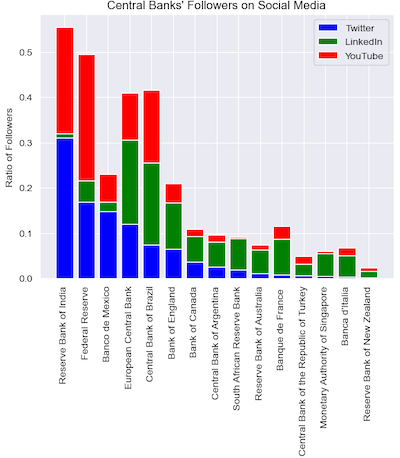
\includegraphics[width=\linewidth]{0-banks_followers_ratio.png}
	\caption{}
	\label{fig:followers_ratio}
\end{figure}

Despite the increasing use of social media by central banks, little is known about how their communication strategies on social media impact public perception and market reactions. In this project, we aim to investigate the sentiment of central banks' communication strategies on Twitter and their impact on public perception. By using data science techniques, we will analyze the Twitter networks associated with three central banks: the European Central Bank (ECB), Bank of England (BoE), and Federal Reserve System (FED). We will analyze the sentiment of the tweets and the most discussed topics, as well as the engagement metrics, such as hashtag, retweet, and like metrics, to gain further insights into user engagement. The study will also take a step further to investigate the impact of a significant event,  the "whatever it takes" speech by ECB Ex-President Mario Draghi, on the sentiment of tweets and its correlation with the stock market and as a first 'viral event market manipulator' before the GameStop case. The results of this study aim to provide valuable insights into the communication strategies of central banks and the public's perception of their policies and trust. Moreover, this analysis demonstrates the potential of social network techniques in analyzing  data for understanding public opinion on economic policy issues.


%------------------------------------------------


\section{Central Banks in the Twittersphere:}


The presence of central banks on social media platforms has increased significantly in recent years, with Twitter being the most popular and frequent choice. Among the G20 countries, the European Central Bank (ECB), Bank of England (BoE), and Federal Reserve System (FED) have emerged as the most prominent central banks on Twitter, with a large following and high levels of engagement and is for this reason that our analysis will main foucus on Twitter and on ECB, BoE and FED.

\begin{figure}[ht]\centering
	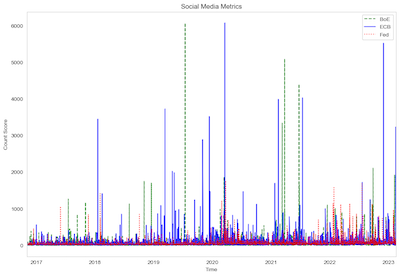
\includegraphics[width=\linewidth]{1-socialmedia_metrics.png}
	\caption{}
	\label{fig:sm_metrics}
\end{figure}

As shown in Figure \ref{fig:sm_metrics} , the social media metrics of these three central banks have shown a clear upward trend over the years. After 2019, due maybe to the COVID-19 pandemic, they started to have more peaks of count score that never stopped showing up again. However, with this increased presence comes the question of the neutrality of these institutions during the social era.

Before to answer this question, is necessary to present a comprehensive analysis of the Twitter networks associated with ECB, BoE, and FED so in this section, we'll introduce two subsections to provide a better understanding of the network graph explorations and clustering of the data we will be talking about.



\begin{figure*}[ht]\centering % Using \begin{figure*} makes the figure take up the entire width of the page
	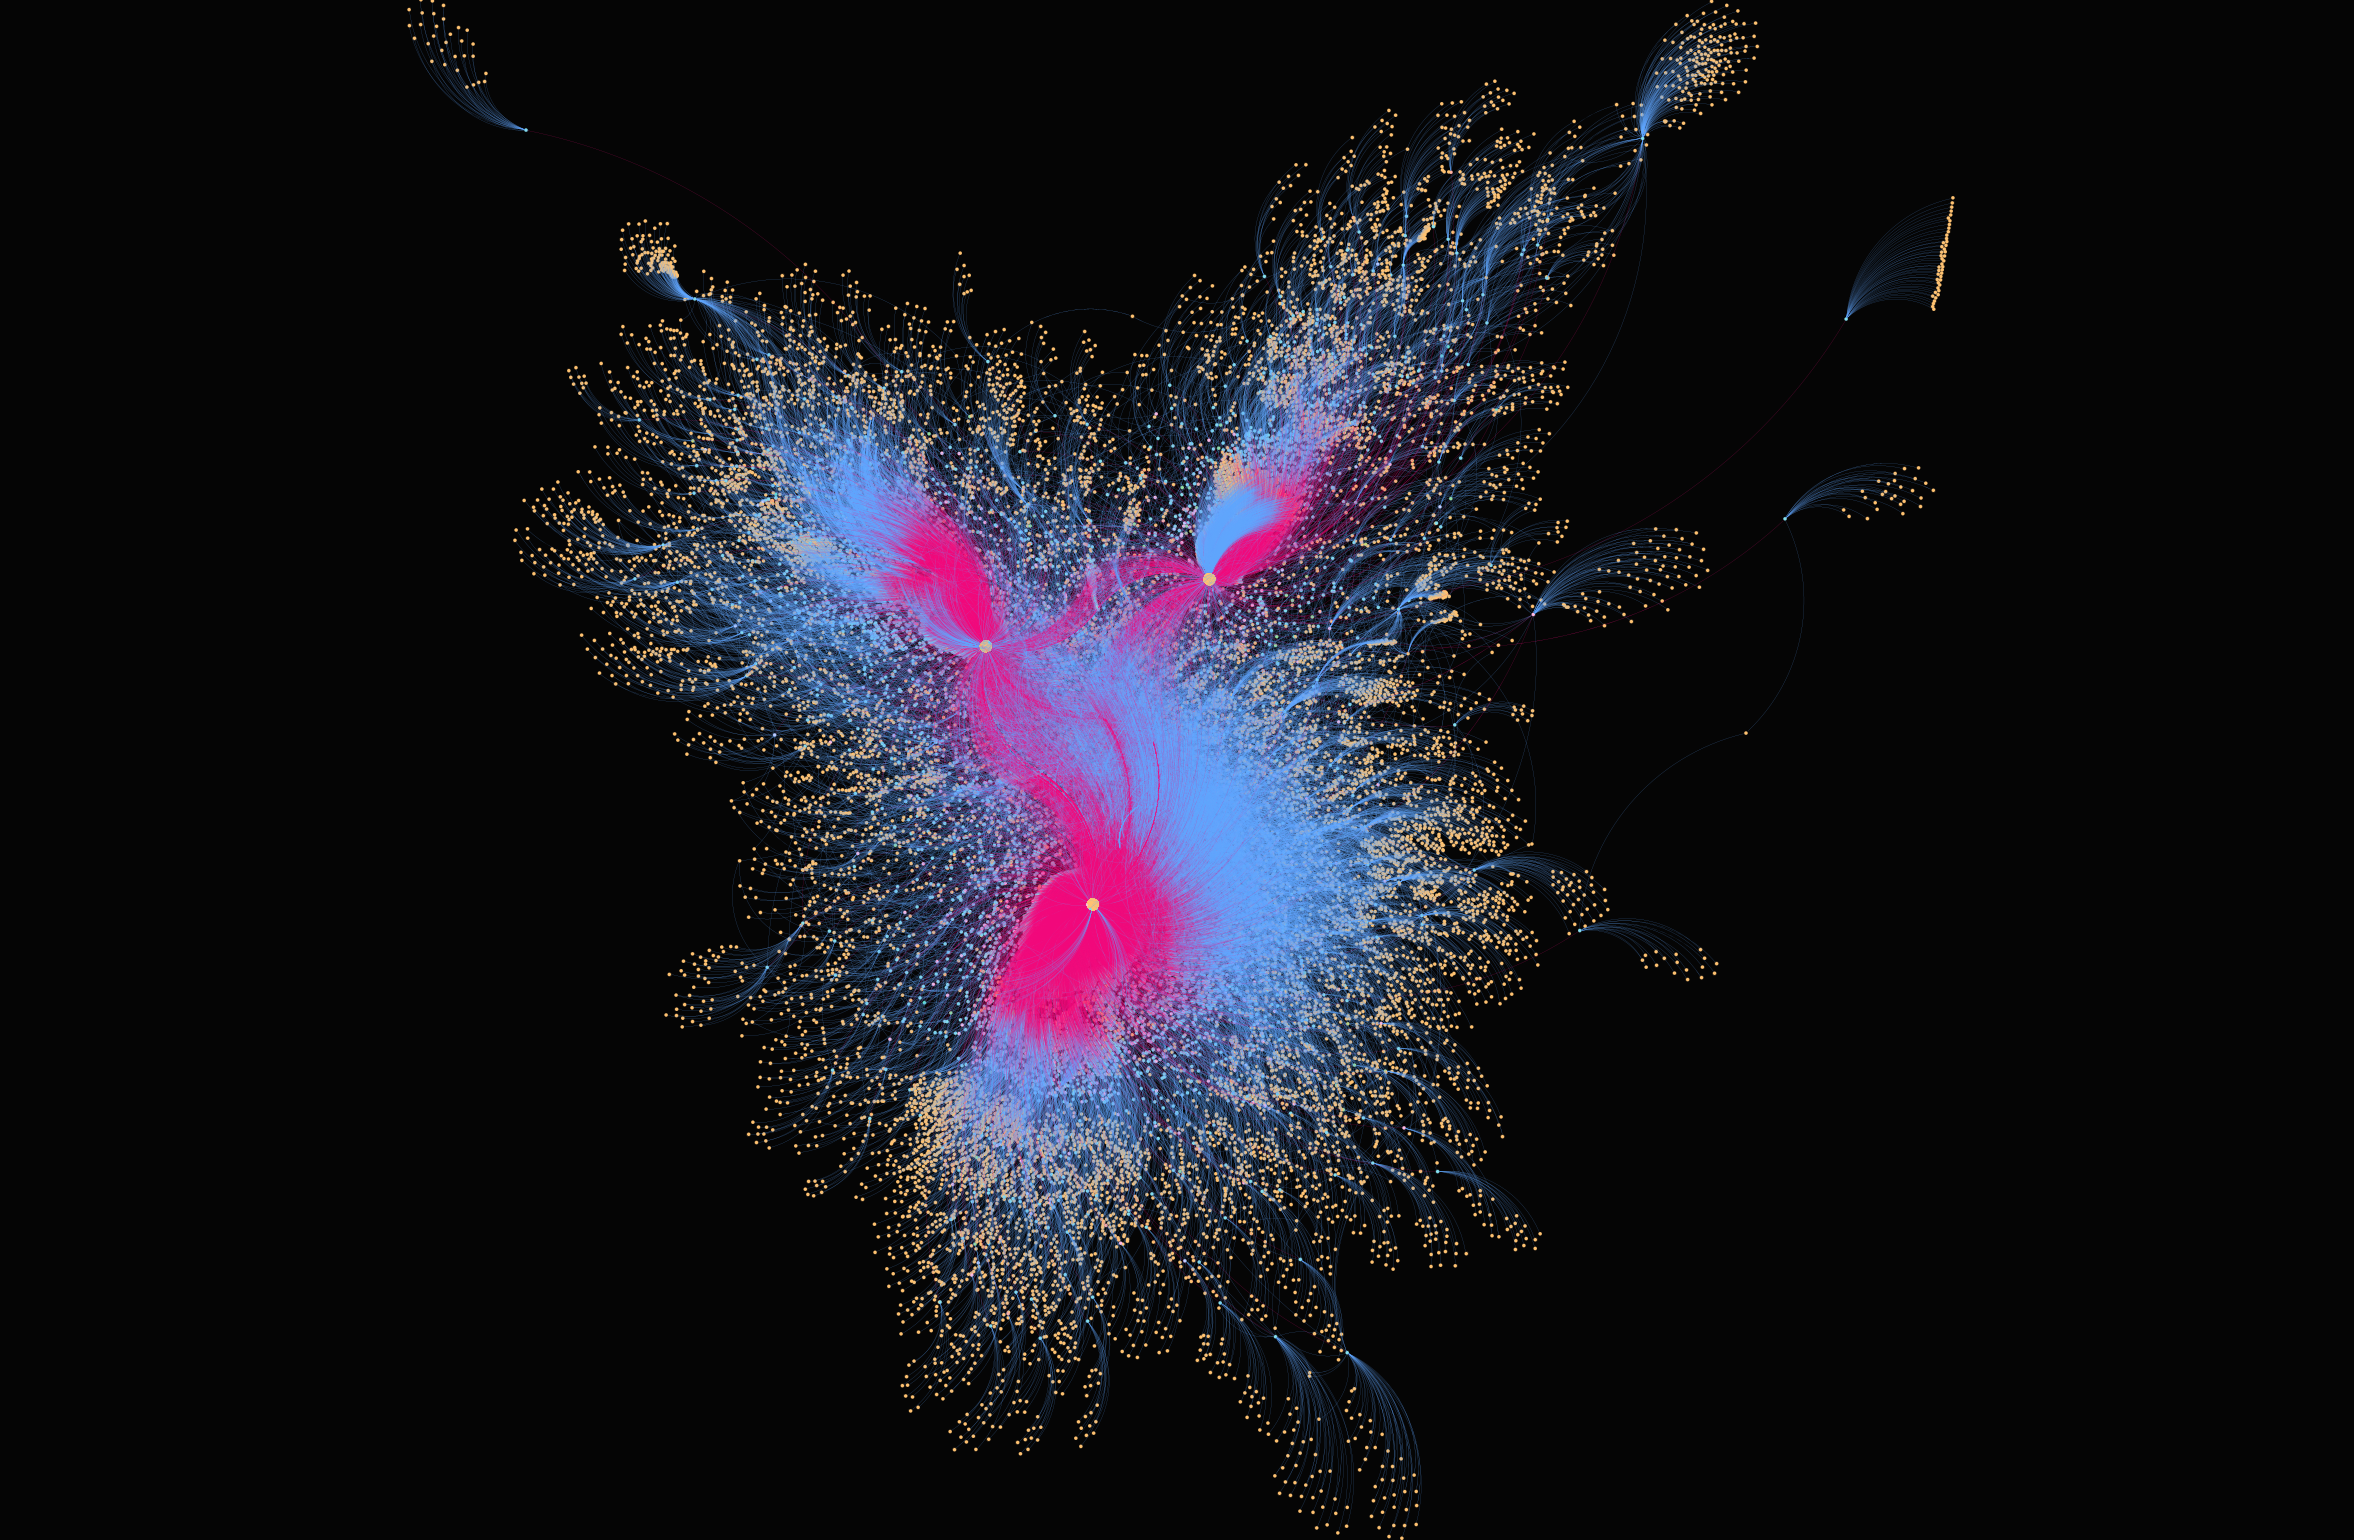
\includegraphics[width=\linewidth]{ntw_graph.png}
	\caption{ECB, BoE, FED gephi network. Please click \href{https://andreramolivaz.github.io/CT0540-graph/}{\textcolor{blue}{here}} for the link of the same graph exported in sigmajs, it will have less quality but still useful for clustering, interaction and descriptions (i.e. Degree, Betweenness Centrality) otherwise consider the gephi file in the zip.}
	\label{fig:ntw_graph}
\end{figure*}

\subsection{ Gephi Network Graph Exploration}

The Gephi Network Graph Exploration (see Figure \ref{fig:ntw_graph}) is an important section of this research as it provides a visual representation of the connection between the ECB, BoE, FED, and their followers, tweeters, and mentions on Twitter. 
The network graph is built using Gephi, a powerful tool for visualizing and analyzing complex networks, and it includes a total of 63590 nodes, where each node represents a different user on Twitter, and 91519 edges that represent the type of connection among users.
The network graph is a valuable resource for understanding the theoretical aspects of how information is shared, disseminated, and communicated among the central banks and their followers. The nodes' attributes include whether they are a bank, influencer, or viral, the language they use, their profession and hashtags made while the edges' attributes include the weight and the type (tweet, follows and mention).
The different colors of nodes are based on the professions of the users, while the colors of edges are given according to the type attribute.  The Gephi network graph allowed for a more in-depth exploration of the Twitter networks associated with the ECB, BoE, and FED. In addition to the previously mentioned attributes, Gephi automatically calculates various metrics for each node in the network, including degree, closeness centrality, and betweenness centrality.

The degree of a node is the number of connections it has to other nodes in the network. In this case, the degree of a user node represents the number of followers, mentions, and tweets it has in relation to the other nodes in the network. The eccentricity of a node is the maximum distance between that node and any other node in the network. This measures how far a node is from the other nodes in the network.

\begin{equation}
	C_D(p_i)=\displaystyle \sum_{k=1}^N a(p_i,p_k) 
	\label{eq:refname2}
\end{equation}


Closeness centrality (in our case for undirected graph) is a measure of how quickly a node can reach all other nodes in the network. It is calculated as the inverse of the average shortest path length from the node to all other nodes in the network. A node with a high closeness centrality is able to quickly disseminate information to other nodes in the network.

\begin{equation}
	C_C(i)=\frac{(n-1)}{\displaystyle \sum_{j=1}^N d(i,j)}
	\label{eq:refname2}
\end{equation}


Betweenness centrality measures the extent to which a node lies on the shortest path between other nodes in the network. It is a measure of the node's control over the flow of information in the network. A node with a high betweenness centrality is able to control the flow of information and exert a significant influence on the network.

\begin{equation}
	C_B(i)=\displaystyle \sum_{j<k}\frac{p_jk(i)}{p_jk}
	\label{eq:refname2}
\end{equation}


The network graph showed that the three central banks had the largest number of connections and the highest influence in the Twitter networks associated with them. This highlights the importance for central banks to be neutral in their communication on social media, as their words and actions can have a significant impact on the wider network. 


\begin{table}[hbt]
	\caption{Some info}
	\centering
	\begin{tabular}{llr}
		\toprule
		\cmidrule(r){1-2}
		Stat & Value \\
		\midrule
		Avg. Degree & $2,878$ \\
		Weekly connected  & $1$ \\
		Avg. Path length  & $21156078$ \\
		\bottomrule
	\end{tabular}
	\label{tab:label}
\end{table}

The network graph's technical aspects and additional stats provide a clear understanding of the theoretical and practical implications of the data. By analyzing the network graph, we can understand the level of engagement of the central banks on Twitter cen be really important and impactful.  It is now important more than ever to try to analyze pattern, sentiment and topic discussed among users to better gain valuable insights into the communication strategies of the central banks on Twitter and their impact on the public's perception of their policies.



\subsection{Clustering}


As mentioned before, nodes have several attributes iincluding "isBank" and "professions". These are two discriminatory values that help us better understand the nature of our network. The first one is used to emphasize our three banks by augmenting the size of their nodes if the twitter user is a bank, while the second one is used to identify the type of audience that the three banks are referring to by creating some clusters.Theclusters created are:
\begin{itemize}[noitemsep] % [noitemsep] removes whitespace between the items for a compact look
	\item politician: red
	\item financial expert: pink
	\item analyst: light-green
	\item curious: ciàn
	\item conspirator: grey 
	\item critic: dark-green
	\item supporter: purple
	\item inestimable: orange
	\item unknown: light-blue
\end{itemize}
All these values are based on the type of tweet that the user tends to make. A function collects keywords of all tweets made, and at the end, it evaluates the "type" of the user. Unfortunately, as we can see from the network graph, most of our users are unknown. This is because our function was not able to classify these users, and another big part of them are inestimable due to the lack of data regarding these users. These are mainly followers, and the data retrieved through API from them was only the username. However, this classification helps us distinguish and detect the main audience of our network.For sure further implementation can be done like for example training a Support Vector Machine (SVM) algorithm to better predict the type of user. However, this was not the subject and main goal of this project.

It is also worth highlighting that edge colors in reverse are based on the type of connection:
\begin{itemize}[noitemsep] % [noitemsep] removes whitespace between the items for a compact look
	\item tweet: red
	\item follow: grey
	\item mention: light-blue
\end{itemize}
The main direct connection from the banks to users is, for sure, tweets, but follows and mentions also play an important role when we talk about virality, diffusion of opinions, and the spread of ideas(ps. the follow plotted are not all of them, we are looking just to a subplot). The network is deeply connected, and a lot of triadic closure can be easly crated. In summary, the clustering technique used here provides us with valuable information about the nature of the network and the type of audience that the three banks are referring to. It is also important to highlight that the clustering technique used in this project can be applied to other social networks (i.e. Youtube and Linkedin two complete different platform with complete different audience), providing new valuable insights into communication strategies and the public's perception id different purposed based social media.

\section{Tweets Evaluation}
This section is the critical and core stage in this project. It aims to evaluate the sentiment of tweets related to the three central banks. To get the required data, we used the snscrape library, which helped to retrieve all tweets related to the official usernames of the ECB, BoE, and FED, as well as their respective hashtags. The tweets were collected from 2021-07 until 2022-07, and all tweets from the given period were preprocessed before any analysis was carried out. The data collected from each tweet include conversation\_id , username, tweet\_text , tweet\_date , retweet\_count , like\_count , view\_count , cash\_tags , hashtags, mentioned\_users , quoted\_tweet , place, vibe, and card. These values are essential for analyzing the sentiment of the tweets and understanding people's perception of the central banks.


\begin{figure}[ht]\centering
	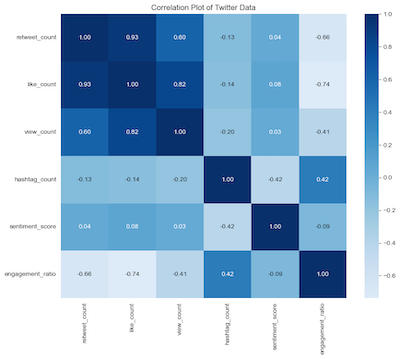
\includegraphics[width=\linewidth]{2-correlation_plot-data.png}
	\caption{}
	\label{fig:crltn_plot}
\end{figure}



The heatmap in Figure \ref{fig:crltn_plot} represent the correlation between the principal data retrieved from each tweet. The heatmap helps us to identify patterns and correlations between the different attributes of the tweets and, doing so, it helps us to identify patterns and relationships within the data, making it easier to us to focus more on the main values that will really useful for our analysis. In this case the main correlated are: hashtag, retweet, like and view. For this reason the next steps necessary to evaluate our tweets will be Sentiment Analysis (based on text and like), topic modelling (based on text ot the tweet and retweet) and finally hashtag interpretation (based on sentiment, hashtag and frequency of hashtag)



\subsection{Sentiment Analysis}

The first section aims to analyze the sentiment of the tweets made by a given user. This is achieved through Natural Language Processing (NLP) techniques that involve preprocessing the tweet text, applying a sentiment analysis algorithm, and creating custom sentiment dictionaries for finance, economics, and banking.The analysis begins by reading and cleaning in the csv file containing the tweets and lowercasing the tweet text. Stop words are removed, and lemmatization is applied to reduce the words to their root forms.Next step include a sentiment analyzer from the Natural Language Toolkit (NLTK) in order to analyze the sentiment of each tweet. The sentiment scores are then augmented using custom sentiment dictionaries specific to finance, economics, and banking. The final sentiment label is determined based on a threshold compound score of 0.05 and -0.05 for positive and negative labels, respectively.

As we can see below the main visualizations generated from the sentiment analysis are histograms and scatterplots showing the distribution of sentiment scores and the sentiment scores over time. Additionally, a bar chart showing the frequency of different emotions in the tweets is also generated. All this visualization technniques provides valuable insights into the users's overall sentiment and emotional state, which is then used to compare the sentiment of each bank from their personal account and the overall sentiment for the 3 banks. 
\paragraph{Sentiment analysis from ufficial account}

\begin{figure}[ht]\centering
	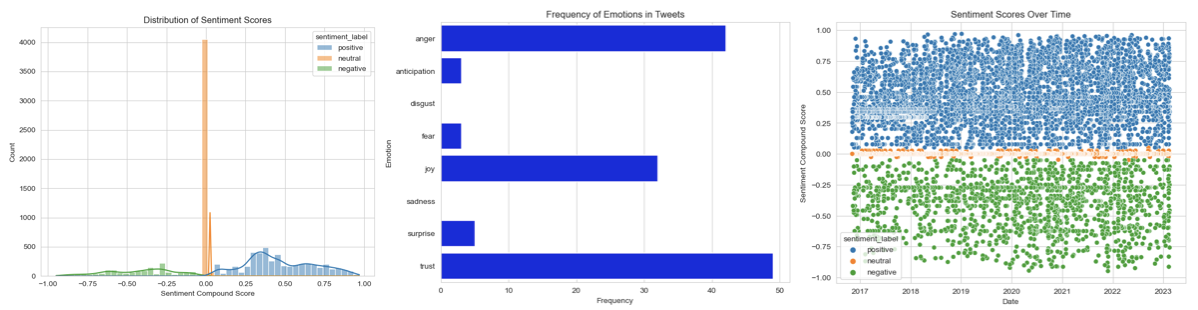
\includegraphics[width=\linewidth]{ecb_stmnt}
	\caption{ECB}
	\label{fig:ecb_stmnt}
\end{figure}

\begin{figure}[ht]\centering
	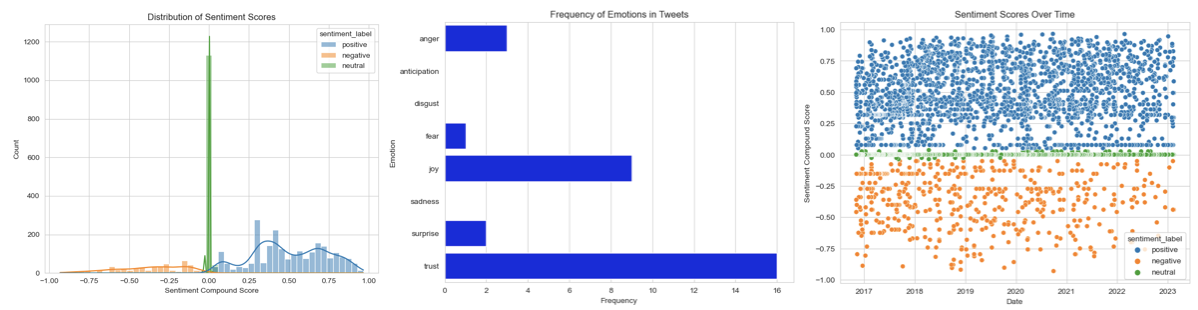
\includegraphics[width=\linewidth]{boe_stmnt}
	\caption{BoE}
	\label{fig:boe_stmnt}
\end{figure}

\begin{figure}[ht]\centering
	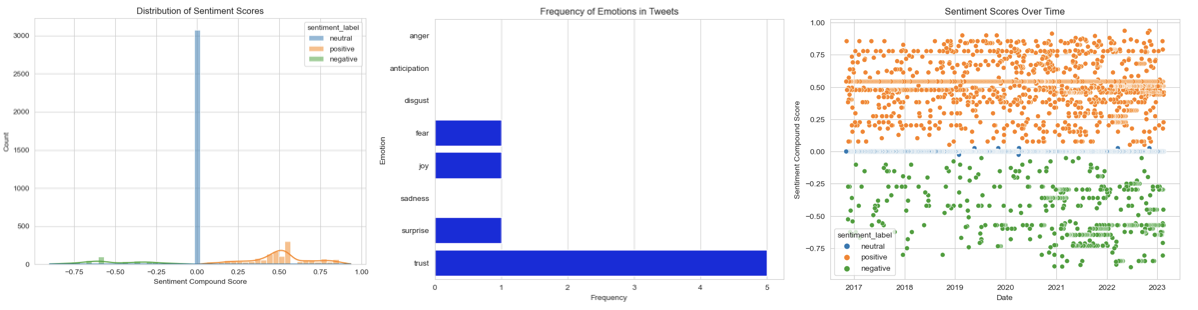
\includegraphics[width=\linewidth]{fed_stmnt}
	\caption{FED}
	\label{fig:fed_stmnt}
\end{figure}


The technical analysis of the graphs plotted for each official account reveals that the sentiment that official banks want to spread among users is largely neutral. The histogram for the ECB (Figure \ref{fig:ecb_stmnt}) shows that negative sentiment is low, with a range of 0 to 250, and positive sentiment is also relatively low, with a range of 10 to 490. The neutral sentiment, on the other hand, is quite high with a count of over 4000. Similar data histograms are plotted for BoE and Fed (Figure  \ref{fig:boe_stmnt}, Figure  \ref{fig:fed_stmnt})and similar intepretation can be made. The distribution plot of sentiment scores over time confirms the previous histogram by highlighting when more positive and negative sentiment were detected, but still shows that the main concentration is on the neutral sentiment for all three banks. The emotions bar chart shows that for each central bank, the most emotions detected are trust, followed by surprise, joy, and fear. Anger is also detected frequently for the ECB, but not as much for the other banks. The data is interpreted as showing that the central banks are striving for neutrality in their communication strategies. This is not surprising given the importance of maintaining confidence and trust in the central banking system. However, the detection of anger on the emotions plot for the ECB is interesting and may be related to historical events such as the eurozone crisis and the subsequent austerity measures.

\paragraph{Sentiment analysis from users}


\begin{figure}[ht]\centering
	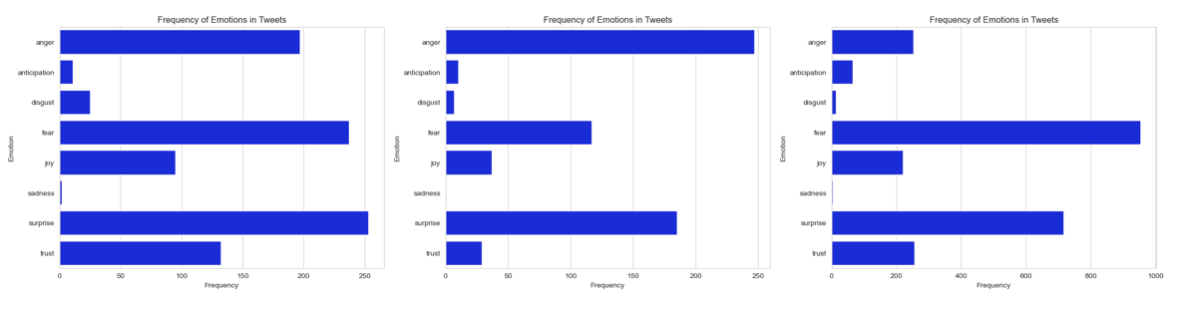
\includegraphics[width=\linewidth]{all_stmt}
	\caption{(ECB - BoE - FED) general emotions detected}
	\label{fig:ecb-boe-fed_stmnt}
\end{figure}


If we rerfer to all tweet related to the 3 banks and not olny from officials account, in reverse the barplot of emotions at Figure \ref{fig:ecb-boe-fed_stmnt} for all tweets related to the three banks (so the network at Figure \ref{fig:ntw_graph} ) shows that fear, anger, and surprise are the most detected emotions, while trust is not among the top emotions detected. This could be because tweets related to banks tend to be negative or critical, given the public perception of banks as profit-driven entities that may not always act in the best interest of their customers. The higher detection of fear could be linked to the general public's anxiety about economic instability, inflation, and job security, which are issues that central banks are responsible for even banks tend to avoid such situations. Similarly, anger could stem from frustration with economic policies or decisions made by central banks that may not align with the interests of the public. The detection of surprise may indicate unexpected events or actions by the central banks, such as policy changes or economic indicators that deviate from expectations.It's also important to note that the sentiment analysis for all tweets related to the banks is influenced by a wider range of factors beyond official communications, such as news articles, public opinions, and market trends and not only tweets. 

\subsection{Topic Modeling}

Now let's continue our analysis and go deeper to see what are the main topics discussed in the tweets. Topic modelling is a widely used technique in natural language processing to extract the main topics from a large corpus of text. In this stage,  has been necessary to use Latent Dirichlet Allocation (LDA) to identify the main topics discussed in the tweets.More in details, after loaded the tweet data and preprocessed the text by converting it to lowercase, tokenizing the text, removing stop words, and removing punctuation, a dictionary is created for all the tokens in the dataset, and low-frequency and high-frequency words are filtered out. After creating a bag-of-words corpus for each tweet, our LDA model is built with ten topics. The LDA model then extracts the main topics and their corresponding top words.  To better visualize the final topics we create a network graph that shows the relationships between the topics and their top words. The node size represents the weight of the word in the topic, and the edge weight represents the weight of the word in the topic compared to the other topics.

In the next section, we will be visualizing the three network graphs to gain insights into the main topics discussed in the tweets for the ECB, FED; BoE and finally we will compare all of them in a unique network graph.

\subsubsection{ECB}

\begin{figure}[ht]\centering
	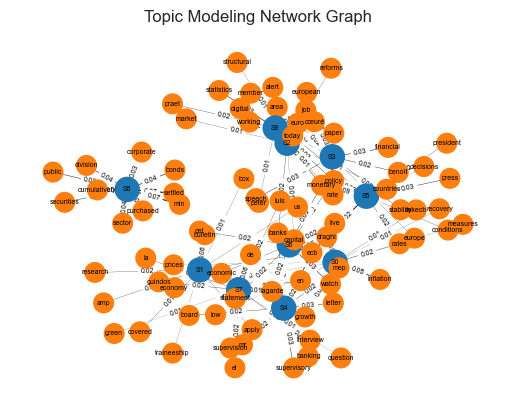
\includegraphics[width=\linewidth]{ecb_topic_modeling.png}
	\caption{}
	\label{fig:ecb_topic}
\end{figure}
Figure \ref{fig:ecb_topic} show the weights assigned to each word in the topics S0 to S7. Each topic represents a specific theme discussed in the ECB's tweets, and each word in the topic is assigned a weight based on its importance in that topic. For example, in topic S0, the words "purchased," "cumulatively," "settled," and "mln" have the highest weights, indicating that these words are the most important in this topic. This topic may be related to the ECB's purchases of financial assets and their settlement process. Similarly, in topic S3, the words "alert," "policy," and "monetary" have the highest weights, suggesting that this topic is related to the ECB's monetary policy and its impact on financial markets.

\subsubsection{FED}

\begin{figure}[ht]\centering
	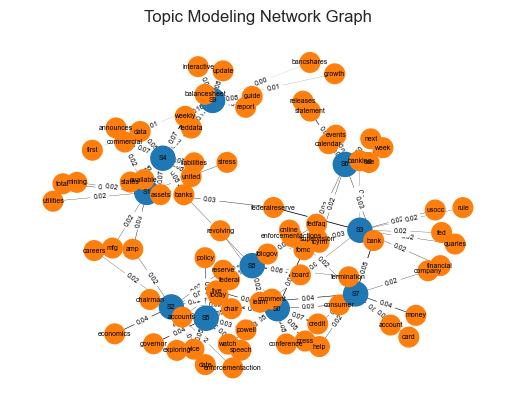
\includegraphics[width=\linewidth]{fed_topic_modeling.png}
	\caption{}
	\label{fig:fed_topic}
\end{figure}

For the Federal Reserve (Figure \ref{fig:fed_topic})tweets, the most important topics based on weight are S1, S2, and S4. Let's analyze the word connections in these topics. For S1, the words "report", "feddata", "guide", "interactive", "weekly", and "balancesheet" are all highly weighted. There seems to be a connection between these words, suggesting that the topic is related to weekly reports and data from the Federal Reserve. For S2, the words "credit", "consumer", "revolving", "nonrevolving", and "saar" are highly weighted. These words are all related to credit and financial matters, which suggests that this topic is related to consumer credit and finance. For S4, the words "feddata", "update", "balancesheet", "weekly", "week", and "calendar" are highly weighted. These words are all related to weekly data and updates from the Federal Reserve, which suggests that this topic is related to weekly updates on the Federal Reserve's balance sheet.
The connections between words in the topic networks suggest that the Federal Reserve tweets are focused on providing weekly reports and updates on the Federal Reserve's balance sheet, as well as on consumer credit and finance.

\subsubsection{BOE}

\begin{figure}[ht]\centering
	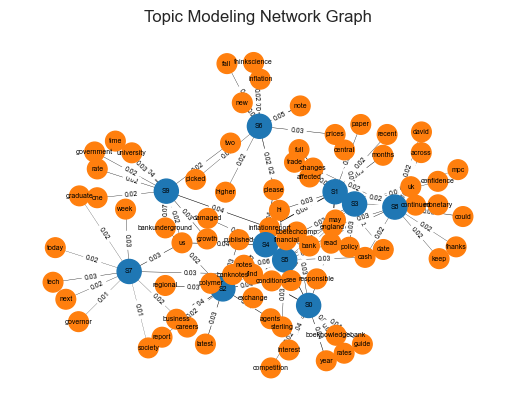
\includegraphics[width=\linewidth]{boe_topic_modeling.png}
	\caption{}
	\label{fig:boe_topic}
\end{figure}


Similary for the Bank of England network (Figure \ref{fig:boe_topic}), we can see that the most important words for each topic are:


\begin{itemize}[noitemsep] 
\item [S0:] policy, costs, monetary, experts, companies
\item [S1:]full, us, boetechcomp, tech, competition
\item [S2:]boeknowledgebank, find, financial, guide, careers
\item [S3:]bankunderground, inflationreport, business, conditions, agents
\item [S4:]inflationreport, read, rates, interest, housing
\item [S5:]responsible, uk, hi, banknotes, royalmintuk
\item [S6:]hi, please, exchange, see, bank
\item [S7:]new, note, hi, polymer, paper
\item [S8:]central, governor, bank
\item [S9:]sterling, cash, import, changes
\end{itemize}

Some of these topics seem to have more specific and clear themes, such as S5 about banknotes and coins or S6 about exchanging damaged notes. However, other topics have less clear themes and seem to be a mix of different concepts, such as S0 or S3. It is also interesting to note that some words appear in multiple topics, such as "banknotes", which may indicate that they are not very specific to a particular topic.

\end{itemize}



\subsubsection{All}

\begin{figure}[ht]\centering
	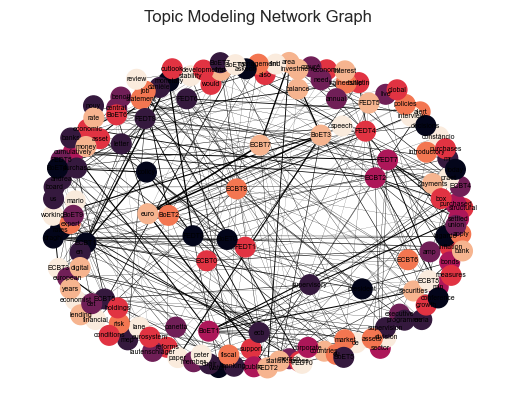
\includegraphics[width=\linewidth]{all_topic_modeling.png}
	\caption{}
	\label{fig:all_topic_corr}
\end{figure}

In this last subsection,ot the topic modeling a final network graph (Figure \ref{fig:all_topic_corr} ) is created that combines the data from the previous three graphs of ECB, BOE, and FED. The utility and functionality of this graph is to provide a comprehensive view of the shared strategies of all three central banks on Twitter. This subsection uses the Fruchterman-Reingold layout to represent the graphs and computes the communities using the Louvain algorithm. Additionally, a matrix of edge weights is created to try to find communities. The resulting network graph has 148 nodes and 300 edges, and provides a clear visualization of the interconnectedness and clustering of topics and users across all three central banks. 
\begin{table}[hbt]
	\caption{Some info}
	\centering
	\begin{tabular}{llr}
		\toprule
		\cmidrule(r){1-2}
		Stat & Value \\
		\midrule
		#Nodes & $148$ \\
		#Edges  & $300$ \\
		Density  & $0.02758$ \\
		isConnected  & $true$ \\
		Avg. shortest path  & $3.9261$ \\
		\bottomrule
	\end{tabular}
	\label{tab:label}
\end{table}





\subsection{Hashtag Interpretation}

The final sub-section of the tweet analysis involves interpreting the hashtags used in the tweets. This analysis as the initial heatmap plotted (Figure \ref{fig:crltn_plot})suggest us,  provides insight into the sentiment analysis. This phase begins by visualizing the top 10 most popular hashtags in the dataset. Next, the frequency of each hashtag over time is calculated and a line graph is created to visualize the trend of each hashtag over time. This provides insight into how the usage of certain hashtags changes over time.

After analyzing the usage of hashtags, sentiment analysis is performed on the tweets. The sentiment of tweets containing each hashtag is calculated and the mean sentiment is computed. This analysis helps in understanding how the public use hashtags, when, the frequency, and the sentiment ralated. Infact, finally, a scatter plot is created to visualize the relationship between hashtag frequency and sentiment score. This helps in identifying any patterns or correlations between the two variables.

\subsubsection{ECB}
\begin{figure}[ht]\centering
	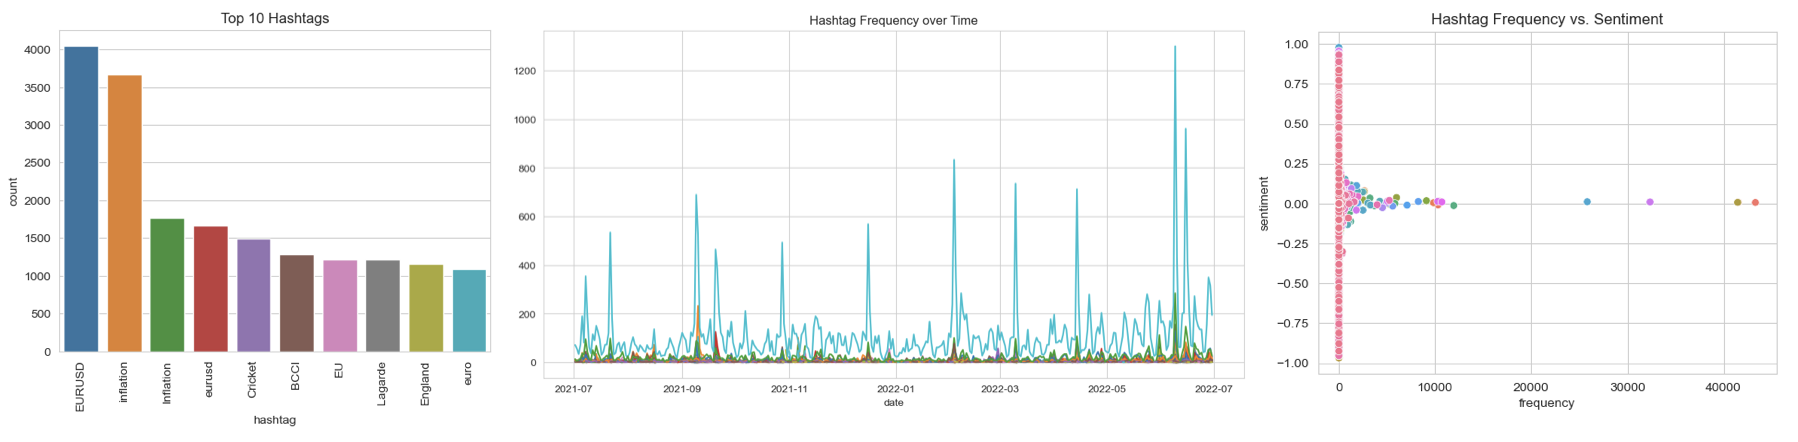
\includegraphics[width=\linewidth]{hshtg_ecb.png}
	\caption{}
	\label{fig:ecb_hshtg}
\end{figure}

The data at Figure  \ref{fig:ecb_hshtg} shows that the ECB's tweets were primarily focused on topics related to the Euro and its relationship to the US dollar (EURUSD), as well as inflation. Interestingly, there are also hashtags related to cricket and the Board of Control for Cricket in India (BCCI), which may suggest some level of noise in the data. The hashtag frequency plot suggests that there were a few specific days where certain hashtags were used more frequently than others due to mabybe some viral event. The sentiment analysis reveals that even though the ECB's tweets may try to be neutral, there are still some tweets with negative or positive sentiment, as seen in the scatter plot. This is the second proof that suggests that even if central banks try to be neutral in their communication, there may still be some subjective interpretations by the public. 

\subsubsection{FED}
\begin{figure}[ht]\centering
	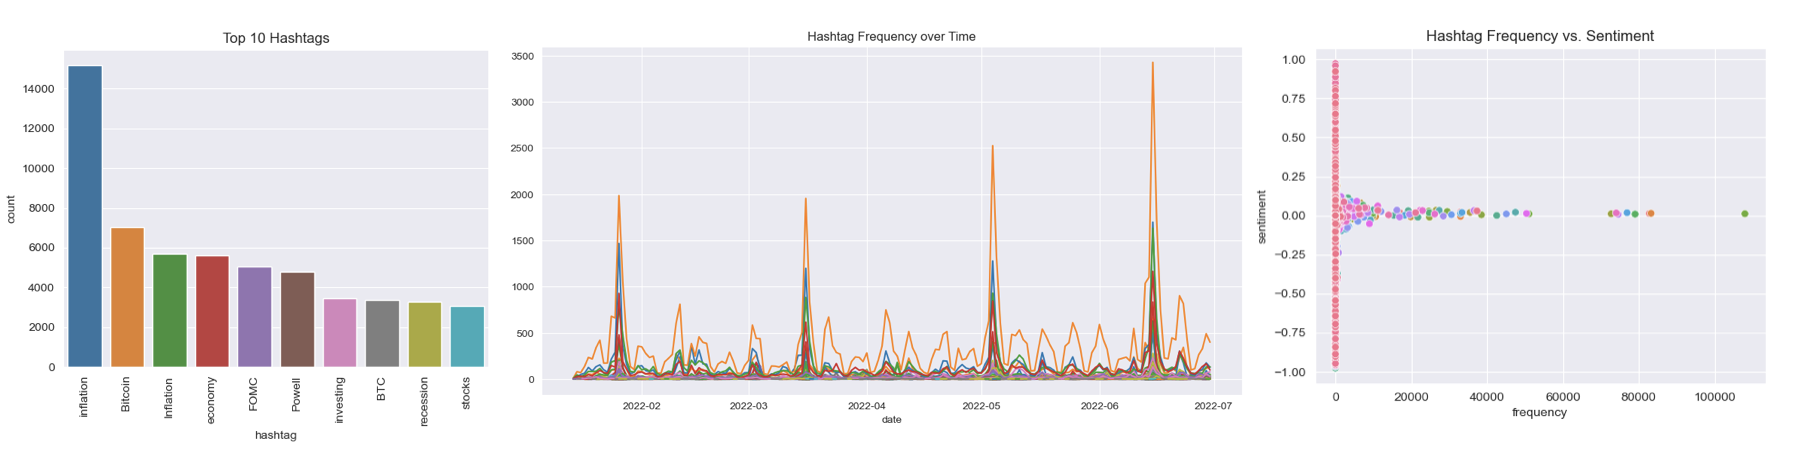
\includegraphics[width=\linewidth]{hshtg_fed.png}
	\caption{}
	\label{fig:fed_hshtg}
\end{figure}

For the FED all hashtags, indicates that there is no clear pattern of sentiment. However, it is interesting to note that the two most frequent hashtags - inflation and bitcoin - have a slightly more negative sentiment compared to the other hashtags, which may indicate a certain level of concern or skepticism among users regarding these topics.In terms of the network graphs, the Fed has a larger and more interconnected network (see Figure \ref{fig:ntw_graph} , the 3 central node are the banks and the the bottom node with more red links is FED ) compared to the ECB and BoE, more data were retrived and so also the scatter plot show more frequent positive and negative outliers. The clusters are also more evenly distributed, indicating a wider range of topics discussed.



\subsubsection{BoE}
\begin{figure}[ht]\centering
	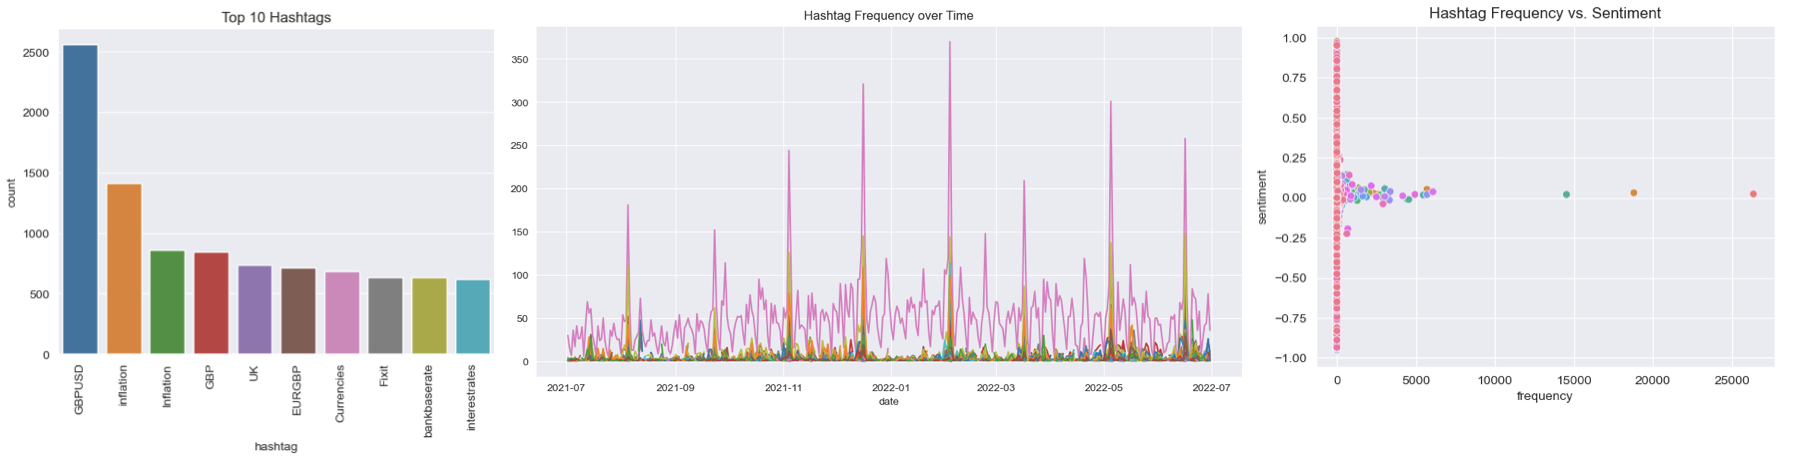
\includegraphics[width=\linewidth]{hshtg_boe.png}
	\caption{}
	\label{fig:boe_hshtg}
\end{figure}


Looking at the BoE graphs (Figure  \ref{fig:boe_hshtg}), we see that the top 10 hashtags clear focus on GBPUSD, GBP, UK, and EURGBP, which suggests that the bank is primarily concerned with the strength of the British pound and its impact on the UK economy. The hashtag frequency graph shows a relatively consistent level of activity with large peaks, which suggests that the BoE's communication strategy is less consistent compared to ECB and Fed. However, there is a small increase in activity around the time of Brexit, which is expected given the significant impact of this event on the UK economy. The scatter plot shows a similar pattern to the ECB and Fed graphs, with sentiment ranging from negative to positive across all frequencies. However, the negative sentiment appears to be more prevalent than in the other two graphs. This could be due to the uncertainty and volatility surrounding Brexit and the impact it may have on the UK economy.

%------------------------------------------------


%------------------------------------------------

\section{Draghi's Speech and Twitter Sentiment}

In this section, we will delve into the impact of Mario Draghi's famous "whatever it takes" speech on Twitter sentiment and the eurozone as a whole. The speech, delivered on July 26, 2012, was a response to the growing concerns about the eurozone's stability and the escalating debt crisis. In the speech, Draghi pledged to do "whatever it takes" to preserve the eurozone and to ensure the stability of the euro currency. These three words sparked a massive rally in financial markets, as investors and traders took Draghi's words as a sign of the European Central Bank's commitment to supporting the eurozone. This is a clear example on how tweets in big networks even if most of the time the sentiment spread is neutral once it change can make a significant impact. To understand the impact of Draghi's speech on Twitter sentiment, we analyzed a dataset of tweets related to the eurozone from 15 days before and 15 days after the speech. 

\begin{figure}[ht]\centering
	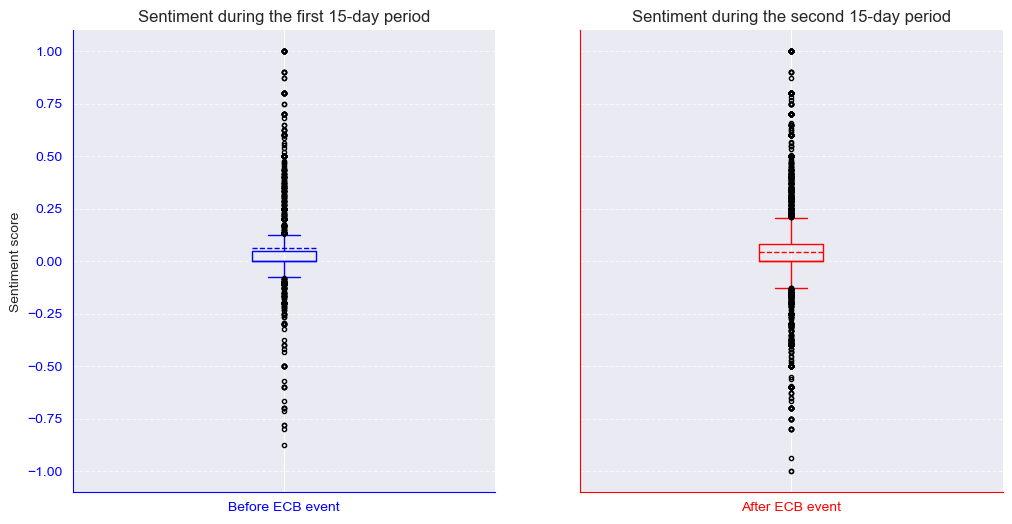
\includegraphics[width=\linewidth]{bxplt.png}
	\caption{}
	\label{fig:boxplt}
\end{figure}



The box plot, labeled at Figure \ref{fig:boxplt}, illustrates the sentiment distribution of the tweets before and after the speech. Before the speech, the majority of the tweets had a relatively neutral sentiment, with a sentiment score falling between -0.07 and 0.12. However, after the speech, the sentiment became more positive, with the median sentiment score remaining the same at 0.07 but the range of scores increasing significantly. This indicates that the speech had a positive impact on public opinion about the eurozone, at least among Twitter users.


\begin{figure}[ht]\centering
	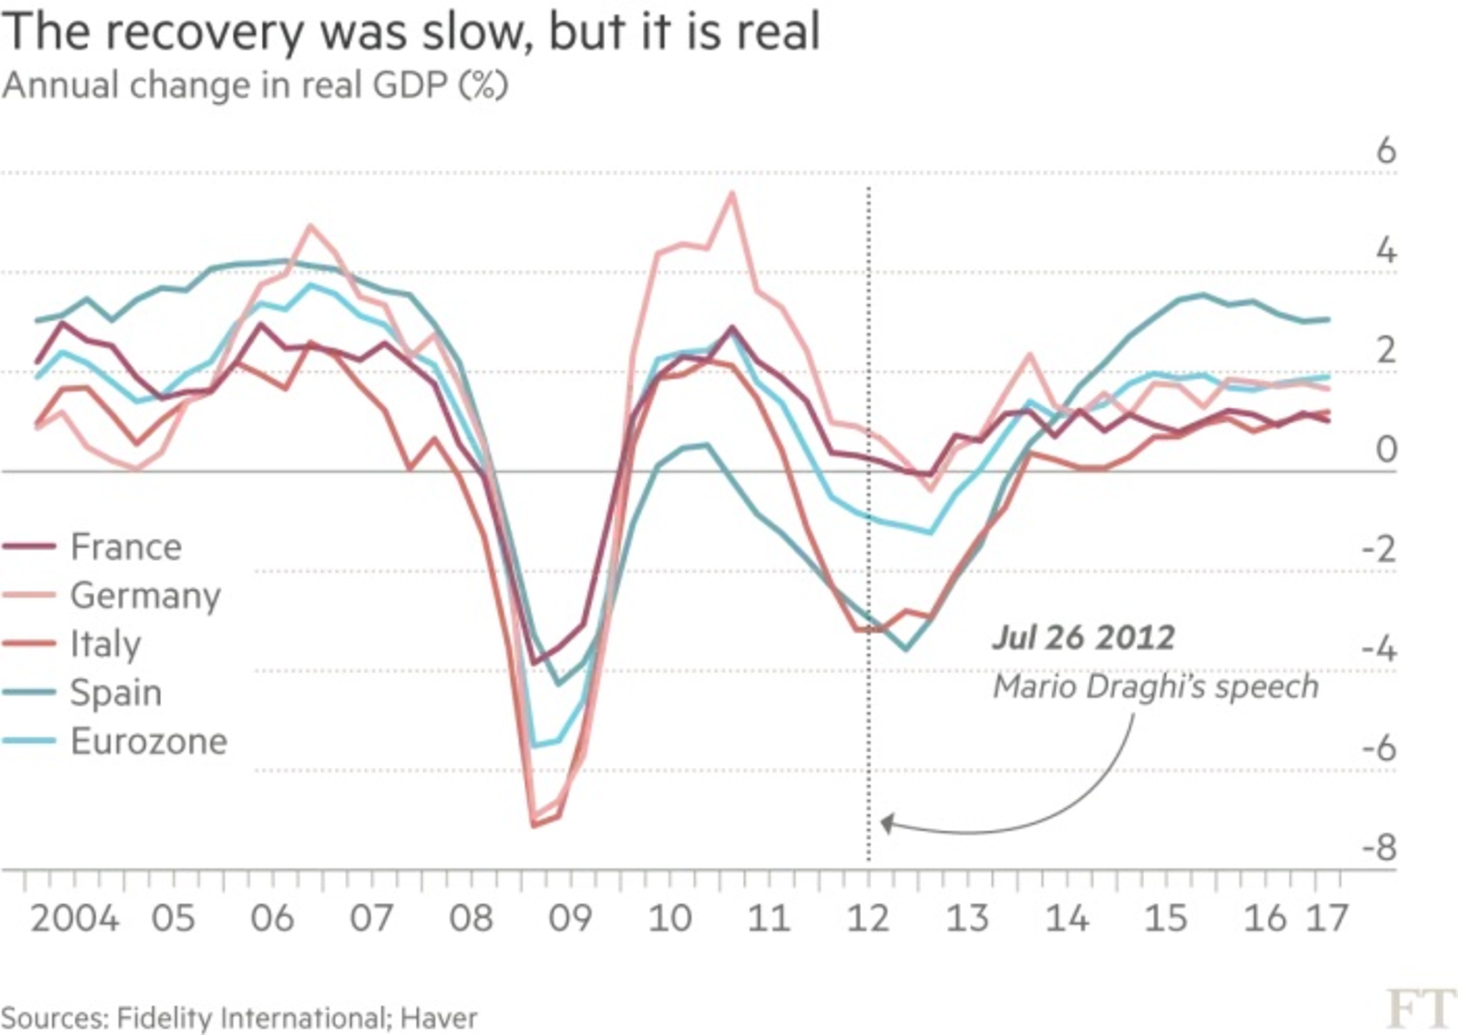
\includegraphics[width=\linewidth]{fncl_time}
	\caption{Source: financial times}
	\label{fig:fncl_time}
\end{figure}

The financial times graph, labeled as Figure \ref{fig:fncl_time}, shows the impact of Draghi's speech on the financial markets. As soon as Draghi delivered his speech, the euro currency rallied, and the eurozone stocks rose sharply. The speech provided a boost of confidence to the markets, and investors became more optimistic about the future of the eurozone. The graph shows a clear upward trend in the euro currency and eurozone stocks after the speech. In conclusion, Mario Draghi's "whatever it takes" speech had a significant impact on Twitter sentiment and financial markets. The speech was a turning point for the eurozone and helped to restore confidence in the region's economy. The sentiment analysis of tweets related to the eurozone shows that the speech had a positive impact on public opinion about the eurozone, while the financial times graph demonstrates the rally in financial markets.






\subsection{Uncovering the Power of Twitter}

In conclusion, our analysis of the social network graphs associated with three major central banks - the ECB, BoE, and FED - has provided valuable insights into their communication strategies and the public's perception of their policies. Through social network analysis techniques, we were able to visualize the network graphs based on followers, tweet mentions, and topics, and leverage sentiment analysis and topic modeling methods to evaluate the sentiment of the tweets and the most discussed topics in each central bank. One key finding from our analysis is the tendency of central banks to maintain a neutral stance in their communication on social media, despite the presence of sentiments among Twitter users that cannot be manipulated. While central banks aim to provide objective and fact-based information, they must also consider the psychological aspect of their communication strategies and how they may be perceived by the public. Another important finding was the impact of significant events on public opinion about the central banks, as seen in the case of Mario Draghi's "whatever it takes" speech. Our analysis revealed that the sentiment on Twitter became more positive after the speech, suggesting that it had a positive impact on public opinion about the eurozone. This demonstrates the importance of understanding the psychological impact of communication strategies in shaping public opinion about central banks.

Overall, our analysis highlights the significance of social media as a platform for central banks to communicate with the public and the need for them to consider the social and psychological aspects of their communication strategies. By leveraging social network analysis and sentiment analysis techniques, our research provides a valuable contribution to the understanding of the complex relationship between central banks and the public in the digital age.

\phantomsection
\section*{References} % The \section*{} command stops section numbering

\addcontentsline{toc}{section}{References} % Adds this section to the table of contents

\begin{itemize}[noitemsep] 
\item [(1)] [CT0540] - Social network analysis: \href{https://www.unive.it/data/insegnamento/339916/programma}{\textcolor{blue}{link}} 
\item [(2)] Learn how to use Gephi: \href{https://gephi.org/users/}{\textcolor{blue}{link}} 
\item [(3)] Publishing interactive graphs online: \href{https://blog.miz.space/tutorial/2020/01/05/gephi-tutorial-sigma-js-plugin-publishing-interactive-graph-online/}{\textcolor{blue}{link}} 
\item [(4)] Snscrape python library: \href{https://pypi.org/project/snscrape/}{\textcolor{blue}{link}} 
\item [(5)] Topic modeling a network approach: \href{https://www.science.org/doi/10.1126/sciadv.aaq1360}{\textcolor{blue}{link}} 
\item [(6)] Basic sentiment analysis with NLTK: \href{https://towardsdatascience.com/basic-binary-sentiment-analysis-using-nltk-c94ba17ae386}{\textcolor{blue}{link}} 
\item [(7)] Detecting community using python louvain: \href{https://stackoverflow.com/questions/53087066/how-to-use-the-communities-module-python-louvain-in-networkx-2-2}{\textcolor{blue}{link}} 






\end{itemize}


\phantomsection
\bibliographystyle{unsrt}
\bibliography{sample.bib}


%----------------------------------------------------------------------------------------

\end{document}